% =============================================================================
% practica1.tex --- Chapter: Practice 1
%
% This file is designed to be compiled either stand-alone (for quick preview)
% or recursively included in the main document.
% =============================================================================

\documentclass[../../__memoria.tex]{subfiles}

\begin{document}
\standalonecover
\pagestyle{cuerpo}

\graphicspath{{\subfix{../../Imagenes/}}{../../Imagenes/}{\subfix{img/}}{img/}}

\chapter[Práctica 1: La Física del AA]{Cuaderno de Laboratorio --- Práctica 1: La Física del Aprendizaje Automático}

\section*{Objetivo}
Comprender la dinámica de la optimización mediante gradiente descendente y el impacto de los hiperparámetros en la convergencia del algoritmo.

% -----------------------------------------------------------------------------
\section[Tarea 1: Tasa de aprendizaje]{Tarea 1 --- Importancia de la tasa de aprendizaje (\texorpdfstring{$\alpha$}{alpha})}
% -----------------------------------------------------------------------------

\subsection{Escenario A (\texorpdfstring{$\alpha_{slow}$}{alpha-slow}): convergencia lenta}
Valor elegido: $\alpha =$ 1e-05\\
\begin{center}
  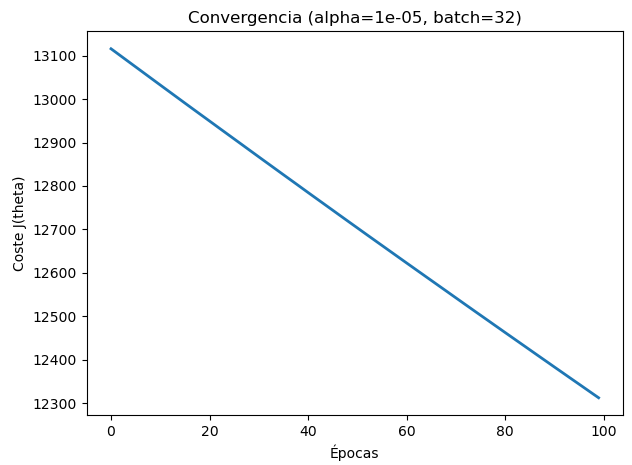
\includegraphics[width=0.85\linewidth]{img/alpha-A-alpha-slow.png}
\end{center}
\textbf{Análisis:} ¿Por qué baja tan lentamente? ¿Cuántas iteraciones estimas para llegar cerca del mínimo?

Baja tan lentamente porque el tamaño de cada paso de actualización es minúsculo (el gradiente del error se multiplica por un $\alpha$ muy pequeño), por lo que los pesos apenas se modifican en cada iteración. Proyectando esta suave pendiente inicial, se estima que harían falta decenas de miles de iteraciones para acercarse de forma significativa al mínimo global.

\vspace{2.0cm}

\subsection{Escenario B (\texorpdfstring{$\alpha_{opt}$}{alpha-opt}): ``curva de codo''}
Valor elegido: $\alpha =$ 0.01\\
\begin{center}
  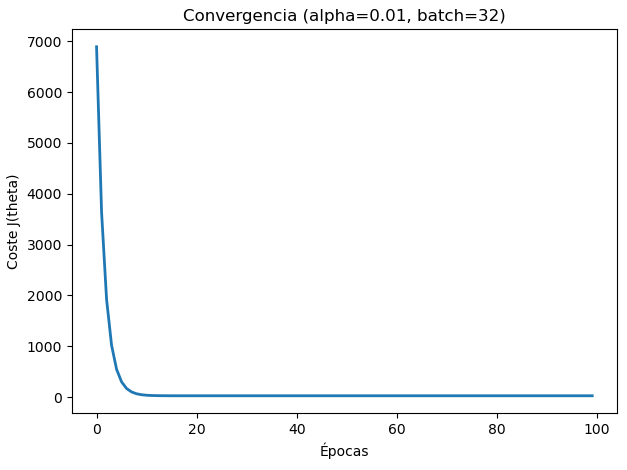
\includegraphics[width=0.85\linewidth]{img/alpha-B-alpha-opt.png}
\end{center}
\textbf{Análisis:} Describe la ``curva de codo'' y qué te indica sobre rapidez y estabilidad.

La ``curva de codo'' muestra una caída inicial muy abrupta seguida de un aplanamiento drástico de la pendiente. Esto evidencia un comportamiento óptimo: el algoritmo avanza muy rápido cuando está lejos del mínimo y, al llegar al fondo del valle, los pasos del gradiente se ajustan milimétricamente sin rebotar, logrando así una gran rapidez en la convergencia y una estabilidad absoluta.

\vspace{2.0cm}

\subsection{Escenario C (\texorpdfstring{$\alpha_{osc}$}{alpha-osc}): oscilación amortiguada}
Valor elegido: $\alpha =$ 0.1\\
\begin{center}
  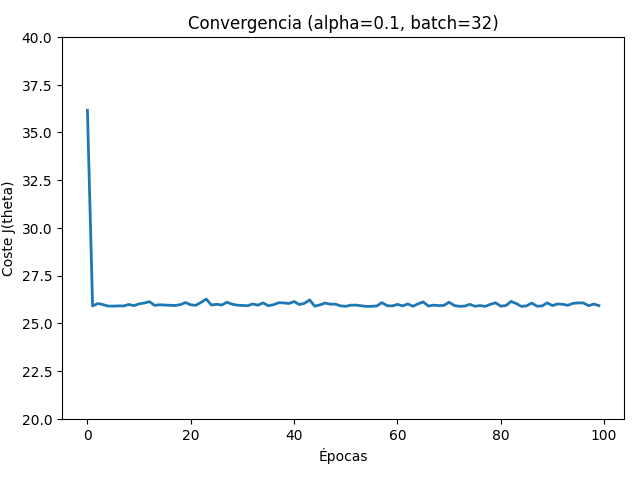
\includegraphics[width=0.85\linewidth]{img/alpha-C-alpha-osc.png}
\end{center}
\textbf{Análisis:} ¿Qué ocurre con $\theta$ en el espacio de búsqueda? ¿Por qué oscila y puede estabilizarse?

En el espacio de búsqueda paramétrica, los pesos $\theta$ están sufriendo desplazamientos de magnitud excesiva y ``saltan'' repetidamente de una ladera a la opuesta del valle de coste, sobrepasando temporalmente el mínimo. Se observan oscilaciones por estos constantes rebotes; no obstante, el sistema logra estabilizarse porque la magnitud del verdadero gradiente disminuye gradualmente, atenuando la amplitud de los saltos hasta converger en la solución.

\vspace{2.0cm}

\subsection{Escenario D (\texorpdfstring{$\alpha_{fail}$}{alpha-fail}): divergencia}
Valor elegido: $\alpha =$ 0.9\\
\begin{center}
  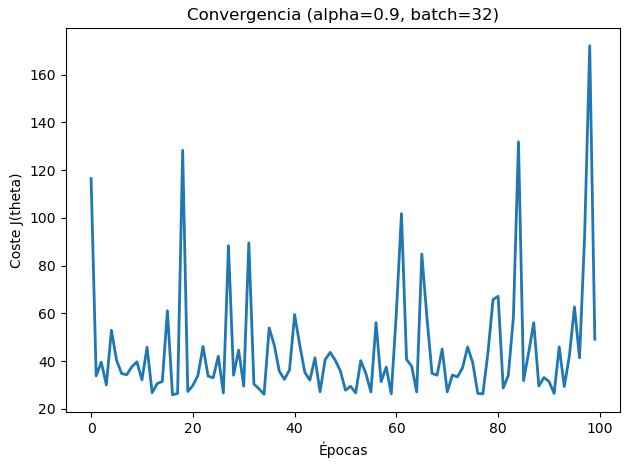
\includegraphics[width=0.85\linewidth]{img/alpha-D-alpha-fail.png}
\end{center}
\textbf{Análisis:} ¿Por qué el error crece? Relaciónalo con ``pasarse'' del mínimo.

El error no deja de crecer porque $\alpha$ es tan grande que cada paso sobrepasa el mínimo por completo. En vez de acercarse, los pesos saltan de un lado al otro del valle, y cada salto es más grande que el anterior. El modelo nunca encuentra una dirección estable de descenso.

% -----------------------------------------------------------------------------
\newpage
\section[Tarea 2: Mini-batch]{Tarea 2 --- Compromiso del mini-batch}
% -----------------------------------------------------------------------------

Usa tu $\alpha_{opt}$ y compara los siguientes esquemas de procesamiento:

\subsection{Batch completo}
\begin{center}
  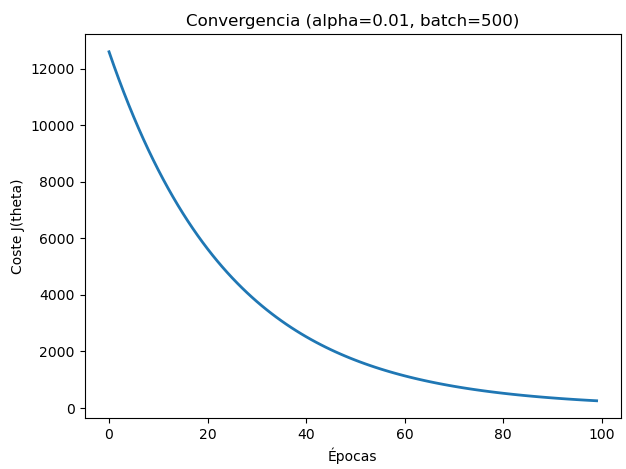
\includegraphics[width=0.85\linewidth]{img/batch-Batch-completo-b500.png}
\end{center}

\subsection{Mini-batch (32 o 16)}
\begin{center}
  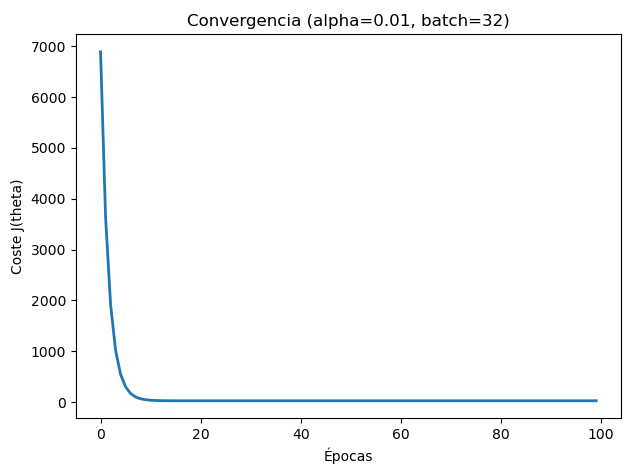
\includegraphics[width=0.85\linewidth]{img/batch-Mini-batch-32-b32.png}
\end{center}

\subsection{Estocástico puro (batch = 1)}
\begin{center}
  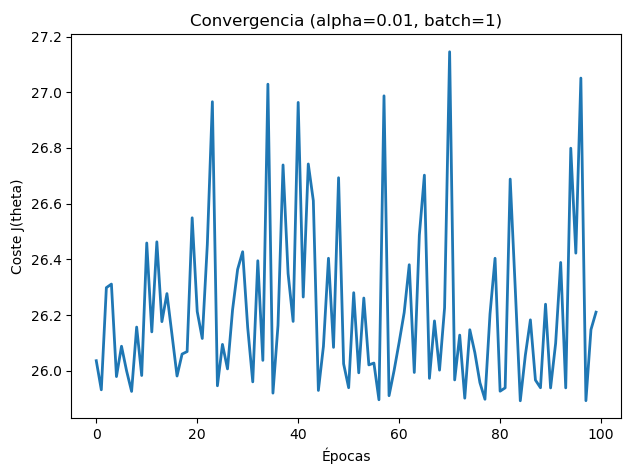
\includegraphics[width=0.85\linewidth]{img/batch-Estocastico-1-b1.png}
\end{center}

\textbf{Preguntas de reflexión:}
\begin{enumerate}
  \item ¿Cuál de las tres curvas es más ``ruidosa'' y por qué?

        La del batch = 1, sin duda. Al calcular el gradiente con una sola muestra, la dirección de descenso cambia constantemente y se ve claramente en la gráfica: la línea tiene picos de subida y bajada continuos. A pesar de eso, a largo plazo la tendencia general sigue bajando.

  \item A nivel de tiempo de ejecución (CPU), ¿cuál ha sido más eficiente? Justifica basándote en computación vectorial.

        Tanto el Batch completo como el Mini-batch son mucho más rápidos que el estocástico porque procesan los datos en bloques y aprovechan las operaciones vectorizadas de librerías como numpy, que internamente trabajan en paralelo a nivel de hardware. En el caso estocástico (batch=1), cada iteración ejecuta un bucle en Python y actualiza los pesos muestra a muestra, lo que multiplica el tiempo de ejecución. Desde mi experiencia, esta diferencia se nota muchísimo: el bucle estocástico tardaba varios segundos mientras que el mini-batch y el batch completo terminaban casi instantáneamente. El \textbf{Mini-batch} me parece el mejor equilibrio porque el descenso es mucho más suave que el estocástico y casi tan rápido como el batch completo.
\end{enumerate}

% -----------------------------------------------------------------------------
% Timing figures --- placed outside the enumerate to maintain correct hierarchy
% -----------------------------------------------------------------------------
\subsection{Tiempo de ejecución --- Estocástico puro (batch = 1)}
\begin{figure}[H]
  \centering
  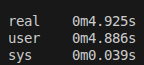
\includegraphics{img/apartado-2-batch-1.png}
  \caption{Tiempo de ejecución con batch=1.}
\end{figure}

\vspace{1cm}

\subsection{Tiempo de ejecución --- Mini-batch (batch = 32)}
\begin{figure}[H]
  \centering
  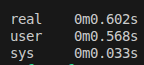
\includegraphics{img/apartado-2-batch-32.png}
  \caption{Tiempo de ejecución con batch=32.}
\end{figure}

\vspace{1cm}

\subsection{Tiempo de ejecución --- Batch completo (batch = 500)}
\begin{figure}[H]
  \centering
  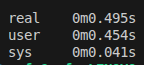
\includegraphics{img/apartado-2-batch-500.png}
  \caption{Tiempo de ejecución con batch=500.}
\end{figure}

% -----------------------------------------------------------------------------
\section[Reto: Criterio de parada]{El reto --- ``Ajuste de precisión'' (criterio de parada)}
% -----------------------------------------------------------------------------

Implementa empíricamente el criterio de tolerancia algorítmica:
\[
  |J_t - J_{t-1}| < 10^{-5}
\]

Para analizar las trayectorias asintóticas del sistema a largo plazo, se estableció un hiperparámetro deliberado que fijaba el límite en 2000 épocas en total. No obstante, al condicionar su diseño algorítmico al criterio de parada $|J_t - J_{t-1}| < 10^{-5}$ y equipar el modelo con su topología inicial más favorable ($\alpha=0.01$, batch$=32$), el algoritmo logra su punto de silla limitante ideal con una prontitud destacable y neutraliza la ejecución sistemáticamente en la \textbf{época 55}, obviando todo cómputo excedente e inútil que le sucediese al modelo a posterior.

\begin{figure}[H]
  \centering
  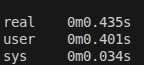
\includegraphics{img/apartad-3-Batch32alfaoptima.png}
  \caption{Tiempo de convergencia interrumpida en la época 55 sujeto a $|J_t - J_{t-1}| < 10^{-5}$ para $\alpha=0.01$ y batch$=32$.}
\end{figure}

% -----------------------------------------------------------------------------
\section[Conclusiones]{Conclusiones}

Lo que más me ha quedado claro después de esta práctica es que el gradiente descendente no funciona por sí solo: hay que ajustar bien los hiperparámetros o el algoritmo no converge o lo hace demasiado lento. 

Con $\alpha$ muy pequeño (1e-5) el error bajaba tan despacio que necesitaba muchísimas iteraciones para acercarme al mínimo. Con $\alpha$ muy grande (0.9) el modelo directamente divergía, y el error se disparaba sin remedio. Encontrar un valor intermedio (0.01) marcó la diferencia: la pérdida caía rápido al principio y luego se estabilizaba sin rebotes. No esperaba que el comportamiento cambiase tanto con solo mover un número.

En cuanto al tamaño de batch, el estocástico puro (batch=1) era tan ruidoso que costaba seguir la evolución del error, y además era el más lento con diferencia. El batch completo era rápido pero el descenso no era tan fluido. El mini-batch de 32 muestras me pareció el punto óptimo: convergía casi igual de rápido que el batch completo, la curva de pérdida era mucho más estable que la estocástica, y computacionalmente era eficiente porque numpy procesa los bloques en paralelo.

Por último, implementar el criterio de parada $|J_t - J_{t-1}| < 10^{-5}$ fue sencillo y resultó muy útil: el modelo dejaba de entrenar automáticamente cuando ya no mejoraba, evitando iteraciones innecesarias. En mi caso, con $\alpha=0.01$ y batch=32 se detuvo en la época 55.

\vspace{3.0cm}

\end{document}
